\chapter{Theoretical Foundations}
In this section, the theoretical foundation of this thesis will be laid to understand the problem and the components used to solve it. First, the dataset KIT-Motion Dataset combines both the motion themselves as xml-Data in the mmm-format, and to each motion, a textual annotation has been assigned. Thus making it semantically rich and allowing natural language processing to be used to solve the problem.
\section{Human activity recognition}\label{sec:HAR}
In the fields of medicine, surveillance, and sports human activity recognition play a great role. Applications of HAR are intra-disciplined and range from surveillance of the elderly to high-performance sports, and quantifying calorie consumption based on the performed human activities. In practical terms, two main paradigms exist in the field of HAR: video-based systems and sensor-based systems\cite{chen2021deep}. In the first approach, videos or still images are used to classify the activity performed in said video or image. On the other hand sensor-based systems, the main focus of this thesis, use the information generated by sensors to perform the task of HAR. The second approach is highly valuable due to the proliferation of sensors in the modern lifestyle, integrated into wearable devices or in portable devices such as smartphones, facilitates the uninterrupted and non-intrusive logging of humans motion information\cite{chen2021deep}.\newline
To implement this, it might be very helpful to use sensors to know the relative position of a body part, its speed, and its acceleration, which is also the base for this thesis. This approach is very promising, due to the prevalent nature of wearables capable of capturing this information. Here, some of the methods used in practice are outlined and the difficulties encountered by researchers to have a picture of the state of the art in HAR and how it was achieved.\newline
\subsection{Approaches to the HAR problem in practice}\label{subsec:approachesHAR}
First, the shape-based methods have received a lot of attention since the 2000s, where the human body is described in 2D space as rectangular patches and as volumetric shapes in 3D spaces. In other words, the human body is reduced to a silhouette consisting of limbs jointly connected. This approach is relevant in classifying human motions captured in videos\cite{vrigkas2015review}. This makes classifying motion captured on videos feasible and proves that temporal-spacial input for classifying motions is relevant for this task. However, the identification of the body parts that contribute the most to the task of activity recognition remains challenging and requires the use of a hierarchical composition model such as in \cite{lillo2014discriminative}. Lillo et al. showed that hierarchical compositional models reach a high level of precision in determining, which actions are performed by a person and the relevant part for it. In addition to that, their model could determine, if a person is performing multiple tasks at the same time, i.e. walking while having a phone call, and could discriminate between actions that can't be performed at the same time. In other words, their model builds a discriminative dictionary of body pose primitives, which are combined to compose atomic actions at a low level. Consequentially, these atomic actions are combined to compose complex activities at the top level\cite{lillo2014discriminative}.\newline
Another approach is using the multimodal methods, which were the focus of recent studies and attempts to tackle this problem. Here, events are seen as an ensemble of values of some descriptors, i.e. the position of the arm and its velocity, in a moment. Thus providing the model with more useful information. However, the collected information should be somehow fused in a meaningful way, thus making feature fusion a necessary tool to achieve this. One can differentiate between two extreme strategies: early and late fusion, though hybrid approaches exist, such as slow fusion and single frame as illustrated in fig \ref{fig:feature_fusion} and explained in more detail in \ref{subsec:feature-fusion}. In the context of classifying human activities by using information about the positions of the joints feature fusion could make the trained models very robust against occlusion and noise and could improve the recognition performance\cite{vrigkas2015review}.
\subsection{Feature Fusion}\label{subsec:feature-fusion}
The need to use feature fusion for the task of human activity recognition is due to the fact, that this can be achieved by using a multitude of inputs, i.g. visual or auditory. In this thesis, only information about the joints and the position of the pelvis is taken into account. However, each joint is positioned on an axis, thus making it useful to use feature fusion in this context. Karpathy et al. investigated fusing information across the temporal domain using multiple methods listed in fig \ref{fig:feature_fusion}. In principle, the fusion can be used in the early stages of a CNN by modifying the first convolutional layer in the network and extending them in time. Another approach is to delay the fusion and replace the first layer with two temporally separate single-frame networks. Later can the fusing of the output of the two single-frame networks take part\cite{karpathy2014large}.\newline
\begin{figure}[H]
	\begin{center}
		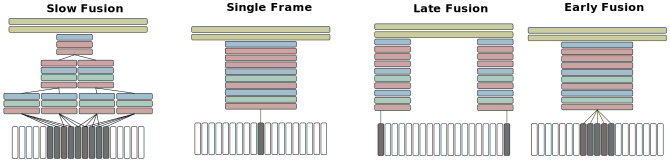
\includegraphics[width=.75\textwidth]{img/feature_fusion.pdf}
		\caption{Representation of fusion of information as shown in \cite{karpathy2014large}}
		\label{fig:feature_fusion}
	\end{center}
\end{figure}
\begin{description}
	\item[Single frame] was used as a baseline to understand the contribution of static appearance to the classification accuracy\cite{karpathy2014large}.
	\item[Late fusion] places two separate single frames with shared parameters at the beginning and the end of a window. Then, their outputs are merged in the first fully connected layer. This allows the model to detect global motion characteristics and makes the classification process more robust, which can be achieved by comparing the output of both single frames\cite{karpathy2014large}.
	\item[Early fusion] is an extension of the single frame architecture, where information is combined across an entire time window. The direct and early extraction of the data would allow the machine learning to detect local motion and speed in a precise manner\cite{karpathy2014large}.
	\item[Slow fusion] fuses temporal information throughout the network and allows higher layers access to global information in both the temporal and spatial dimensions. This can be implemented by extending the connectivity of all convolutional layers and making this architecture a mix of early and late fusion\cite{karpathy2014large}.
\end{description}
\subsection{Some inherent Problems with HAR}\label{subsec:probHAR}
To understand the complexity of the HAR problem, one must understand the problem of recognition. This would allow researchers to understand the intricacies of the problem in general and contribute to unifying the process of developing general recognition systems. As Kaixuan Chen and Dalin Zhang et al. recognized the fact that the challenges faced by HAR are shared by other fields of research such as computer vision and natural language processing\cite{chen2021deep}. Nevertheless, some of these challenges are unique since sensor-based HAR requires dedicated methods for real-life applications.\newline
First in the list comes feature extraction, due to the nature of the HAR, a classification task, it shares this problem with other classification problems. This is the case due to the inter-similarity problem, where multiple activities share some similarities, e.g. walking and running. This makes extraction features that uniquely represent each activity very challenging. In addition to that, generally training robust and performant models requires a huge amount of correctly annotated data. However, collecting and annotating data is costly and time-consuming. This makes annotation scarcity a problem plaguing all domains of research in supervised learning. Moreover, this is further aggravated by the inherent nature of human activities, where some classes are more represented, e.g. walking, sitting, etc..., which is known as class imbalance. In practice, a multitude of methods exists to overcome the challenges related to datasets, such as using a weighted loss function, which penalizes the model during the training more in case of the miss classification of an instance labeled with a less represented class. In addition to that, one can use over-sampling to balance the used datasets by duplicating instances of less represented classes or removing some instances of dominant classes, which must be used sparingly to avoid overfitting\cite{chen2021deep}.\newline
On top of that, the recognition is challenging due to the complexity of data association, which refers to the number of users and activities the data gathered is associated with. This is further the case by sophisticated data association. In practice, activity recognition tasks are primarily based on simple activities. Conversely, the more meaningful way to log human activities is composite activities that comprise several simple activities. An example of that is that hand washing can be expanded into \{turning on the tap, soaping, rubbing hands, turning off the tap\}\cite{chen2021deep}. This makes accurate recognition very challenging due to the need for precise data segmentation techniques. Similarly, concurrent activities pose another problem to accurate recognition and drive up the complexity of HAR tasks.\newline
Lastly, the generation of HAR is linked to privacy issues and data protection regulations. This in part limits researchers' ability to collect and annotate data and makes the development of learning machines in this field more challenging, which is the case for deep neural networks as a result of their black-box nature. In other words, it is very difficult to predict, what the network is going to learn from the data, and this makes it possible that these models might unintentionally learn highly discriminate user-informations. This can increase the danger of information disclosure. However, some approaches were adapted to mitigate this, such as the use of an adversarial training framework as a risk mitigation measure for sensitive/unintended information disclosure\cite{iwasawa2017privacy}.
\section{Natural Language Processing}\label{sec:nlp}
Natural language processing began in 1950 as the intersection of artificial intelligence and linguistics. At first, it was very distinguishable from test information retrieval, where researchers employed highly scalable statistical techniques to index and search large volumes of text in an efficient manner\cite{nadkarni2011natural}. Nowadays the two domains converged to create a new NLP field of study, where researchers are required to borrow from other fields to create new methods of analyzing and interpreting information in a textual or spoken form.\newline
With Chomsky's 1956 theoretical analysis of language grammar, an estimate of the complexity of the problems in NLP was provided and influenced the creation of the Backus-Naur Form. This notation specified context-free grammars and is the base of programming language representations. In addition to that Chomsky found more restrictive Grammars, regular grammars, which are used to specify text-search patterns\cite{nadkarni2011natural}. These constructs were first the base of the first logic programming language Prolog, which syntax was conceived to suit writing grammars.\newline
These approaches in the early days relied heavily on symbolic and hand-crafted rules and didn't contribute to the semantic analysis, i.e. extracting the meaning, but were used to syntactically analyze text and to check the syntactic consistency of programs. Nevertheless, these formal grammars can specify the relationship between text units, and they can be extended semantically by expanding sub-categorization and adding more rules and constraints. However, this leads to an explosion of the number of rules and an unmanageable and unpredictable interactions\cite{nadkarni2011natural}.\newline
In the 1980s, NLP pivoted drastically into a statistical approach outlined by Klein\cite{kleincs}, where using simple and robust approximations as outlined above was replaced by deep analysis with leaning machines, e.g. Transformers..., which used probabilities and were trained by large and annotated corpora. More so, the evaluation of the trained learning machines was more diligent and precise\cite{nadkarni2011natural}. This birthed the model statistical NLP, where the hand-crafted rules were replaced by broader rules having probabilities determined through the trained machine learning\cite{kleincs}. In the practical part of this thesis, some low-level NLP tasks will be used to extract and determine the class of each motion with its annotation. Tokenizers are an example of a low-level NLP task, where the individual tokens, i.e. words, and punctuations, are identified. To achieve this a lexer is used to divide the text into lists of subtexts, that are then used in the next steps of the syntactical and semantic analysis of the text.\newline
A central task in this thesis is the syntactic analysis of texts and speech and assigning to each identified token a tag, i.e. the position and the role in the sentence\cite{nadkarni2011natural}. To this end, Matthew Honnibal implemented a part of speech tagger to tag tokens in a sentence, where he used an averaged perceptron. Here a table of data is provided, but the last column, i.e. the position of each token in the sentence\cite{honnibal_2013}. In addition to that, a stemmer, which can transform tokens into the stem, is important to truly determine the frequency of appearance of a meaning in a text not a transformed version of the word itself. This would work as a categorization process due to the fact that most morphological variants of words have a similar meaning and can be interpreted as equivalent for this purpose\cite{jivani2011comparative}. For this task, a variety of algorithms exists to extract and stemmetize all tokens in a text. 
\subsection{Stemmers}\label{subsec:stemmer}
Stemmers are an important part of any information retrieval systems as well as a common requirement of natural language processing. Its main goal is to transform any word into its root form. In other words, the aim is to reduce inflectional forms and derivationally related forms of a word to a common basic form, that represents the general meaning of it\cite{jivani2011comparative}.\newline
In practice, an abundance of algorithms and methods exists to perform this task and each of these algorithms converts the morphological variants of a word like dance, dancing, danced, etc., and maps them to the word ``dance''. However, some algorithms map these variants to ``danc'', which is correct as long they map them to the same basic form.\cite{jivani2011comparative} Moreover, stemmers can in some cases over or under stem. On one hand, over-stemming is the case when two words with stems are mapped to the same root, and on the other hand, under-stemming is the case when two words with the same stem are mapped to two different stems. Here, Paice distinguished approaches to avoid these stemming errors. The first is to use a light-stemmer, which is geared toward reducing over-stemming errors and as a consequence can make more under-stemming errors. On the other hand, heavy stemmers remove all endings of the processed word, which can be over-corrective in some cases leading to more over-stemming errors. This trade-off must be taken into account while designing a stemming algorithm.\cite{paice1994evaluation}\newline
Stemming algorithms can be classified into three classes, truncating methods, statistical methods, and mixed methods, where each type has a distinct way of mapping words to a stem.\cite{jivani2011comparative}.
\begin{description}
	\item[Truncating methods] as the name suggests remove the affixes(prefixes and suffixes) of a word.
	\item[Statistical methods] are based on statistical analysis and use statistical methods. Most of these methods remove the affixes like truncating methods, but only after applying a statistical process. Examples of such methods are N-Gram Stemmer and HMM(hidden markov model) Stemmer.
	\item[Mixed methods] are hybrid approaches such as Inflectional \& Derivational, Corpus Based and Context Sensitive.
\end{description}
In this thesis, to categorize the motions using the annotation a truncating method was used, namely, the porter stemming algorithm which is one of the most popular stemming methods for the English language. It is based on the assumption that most words in the English language are for the most part made up of smaller and simpler suffixes. It processes words in five steps and in each step rules are applied until one of them passes the condition. The output of the last step is the stem of a processed word. In total, the algorithm checks about sixty rules. To implement this, a framework known as ```Snowball'' was designed to allow users to develop more stemmers geared toward other languages. This stemmer can be classified as a light stemmer, thus allowing for simple and speedy stemming, where the main task is information retrieval not producing correct linguistic results.\cite{jivani2011comparative}
\section{Classification of Time Series}
Time series are ubiquitous and occur in nature in a multitude of ways, such as weather patterns and physiological signals, and also in human activities, such as financial recording. This makes their classification a cross-domain task, with a very strong baseline. Understanding this problem and solving it may influence the domain of machine learning in a significant way\cite{wang2017time}. Recently, it has been demonstrated that data-driven approaches are pivotal for data mining tasks by using deep learning methods and algorithms. A typically used learning machine for this is the ANN(Artificial Neural Network), which has proven to be capable of matching complicated functions leading to its popularity. A very special kind of ANNs is the CNN(Convolutional Neural Network), which has been primarily used for the task of image classification for its ability to extract spatial features. However, the use of CNNs for the task of classification of time series remains very limited and challenging. On the other hand, RNN(Recurrent Neural Networks) are suitable for this task as it effectively uses the temporal nature of time series.\cite{yang2019time}
\subsection{Deep neural networks}\label{subsec:dnn}
In the paper\cite{yang2019time}, a standard baseline is established to exploit deep neural networks for end-to-end time series classification without the need for preprocessing and feature engineering. The authors evaluated a suite of learning machines:
\begin{itemize}
	\item MLP(Multilayer Perception).
	\item FCN(Fully convolutional Network).
	\item ResNet(Residual Network).
\end{itemize}
\begin{figure}
	\centering
	\begin{subfigure}[b]{0.25\textwidth}
		\centering
		\includegraphics[width=\textwidth]{img/mlp.pdf}
		\caption{MLP}
		\label{fig:wang2017timemlp}
	\end{subfigure}
	\hfill
	\begin{subfigure}[b]{0.25\textwidth}
		\centering
		\includegraphics[width=\textwidth]{img/fcn.pdf}
		\caption{FCN}
		\label{fig:wang2017timefcn}
	\end{subfigure}
	\hfill
	\begin{subfigure}[b]{0.3\textwidth}
		\centering
		\includegraphics[width=\textwidth]{img/resnet.pdf}
		\caption{ResNet}
		\label{fig:wang2017timeresnet}
	\end{subfigure}
	\caption{The network structure of three tested neural networks. Dash line indicates the operation of dropout\cite{wang2017time}.}
	\label{fig:wang2017time}
\end{figure}
This comparative study concludes that ResNets and FCNs in pure end-to-end training achieved better performance than COTE(Collective of \\Transformation-Based Ensembles)\cite{2015TSClassificationCOTE}. In addition to that, the use of global average pooling in the convolution layers in the models in the study enabled the exploitation of CAM(Class Activation Map). Thus finding out the contributing regions in the time series to the specific class\cite{wang2017time}. In fig. \ref{fig:wang2017time} the architectures used by Wang et al. are illustrated.\newline
The MLP, as in fig. \ref{fig:wang2017timemlp}, is used as a very rudimentary learning machine and as a gold standard for time series classification. Here they used three hidden layers, each with 500 neurons and ReLU as the activation function. The output layer in this was a softmax layer to ensure the production of meaningful probabilities, i.e the output represents a probability distribution over the different possible classes.\cite{wang2017time} In addition to that, dropout at each layer was used to decrease the possibility of overfitting, thus making the trained model more generalizable.\newline
Next Wang et al. investigated the use of FCN, as in fig. \ref{fig:wang2017timefcn}, which has shown great potential in image segmentation. Here, each output pixel matches the receptive field, thus making the network trainable given the category-wise semantic annotation.\cite{wang2017time}. However, this makes FCNs suitable as a feature extractor, and as in MLP, the final softmax layer is used to generate the probability distribution. As for the architecture itself, it is comprised of three blocks beside the output layer, and each block is a convolutional layer followed by a batch normalization layer and a ReLU activation layer. This isn't the norm, when it comes to this type of architecture, as Wang et al. removed the pooling function altogether to reduce the possibility of overfitting. Besides, batch normalization is used to speed up the conversion and improve generalization. Finally, the output block is a global average pooling layer to reduce the number of weights\cite{wang2017time}.\newline
The final deep neural network investigated was residual networks, which extend the other deep neural network by adding the bypass connection in each residual block, as shown in fig \ref{fig:wang2017timeresnet}. This help in overcoming the problem of vanishing gradients by allowing direct flow of the gradient to the early layers in the network. As such these networks achieve state-of-the-art performance in object detection and other vision-related tasks. Due to the nature of ResNet architecture, one must expect, that trained models based on it might overfit the training data. This is in part due to the fact, that datasets in the field of HAR are relatively small and lack the variance of data points to capture the complex structures with such models. The main components of the ResNet are taken from the FCN, i.e. the convolutional blocks, and staked on each other\cite{wang2017time}.\newline
However, the research in deep neural networks didn't stop here, as these learning machines can't model other problems in practice. To make these models more compatible with the problem of time series classification, one must take the nature of the problem into account. As such learning machines that have a temporal feature baked into them, and would be better suited for the task of classifying motions and activities, if the input is a time series, e.g. outputs of sensors or the shape and position of the joints in the human body. As such recurrent networks would be great for the task at hand.
\subsection{Recurrent Neural Networks}
The intuition behind RNNs is very simple, as their conception is nothing but the extension of normal ANNs, where the concept of unrolling or unfolding illustrates this extension over the time axis. This is shown in fig. \ref{fig:rnn}. This extension allows direct incorporation of the nature of the problem into the learning machine used. In addition to that, the models shouldn't be dependent on the input size, which is the case for leaning machines in \ref{subsec:dnn}. Here, the learning machine is basically a nonlinear dynamical system generally mapping sequences to sequences, where each layer corresponds to a layer in the special deep neural networks.\newline
\begin{figure}[H]
	\centering
	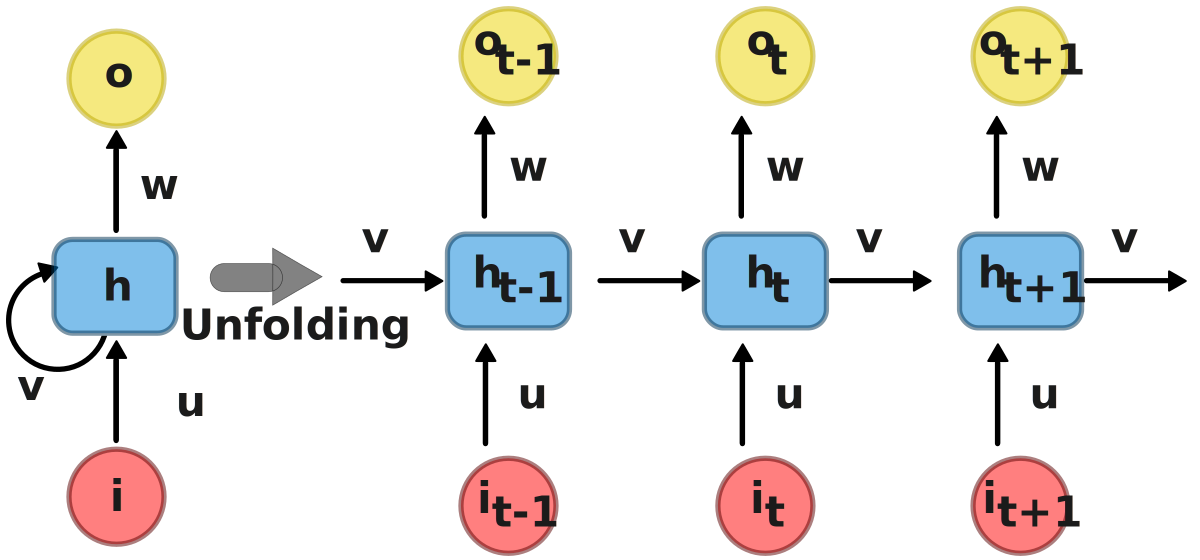
\includegraphics[width=.75\textwidth]{img/rnn.pdf}
	\caption{The recurrent neural network}
	\label{fig:rnn}
\end{figure}
However, the trade-off is having a model that is hard to train, even though the gradient of the network is easy to compute. This is due to the fact, that the nonlinear iterative nature of these models, and that a very minute change to an iterative process can compound and as result lead to a conversely huge change to the results of the later iterations. This in part makes the derivative of the used loss function exponentially large with respect to changes in the hidden states in an earlier time, which results in a very sensitive loss function effectively making it discontinuous. This is severely the case for problems with long-range temporal dependencies\cite{sutskever2013training}. In addition to that, these networks suffer from the vanishing gradient problem, a problem in all very deep neural networks, as it was outlined by Hochreiter in 1997\cite{hochreiter1997long}. In summary, these problems make it very hard to optimize these networks on sequences with very long-temporal dependencies.\newline
Mitigating the vanishing gradient problem is a problem relevant to all very deep neural networks and is a necessity for the training of RNNs. The initial approach would be reducing the number of non-linearities separating the relevant past information from the hidden state of the current recurrent unit. This can be achieved by incorporating direct connections between the past and the current hidden states, which are known as skip connections. The result of using this approach is fewer deep learning problems through reducing the number of non-linearities in the shortest path\cite{hochreiter1997long}.\newline
To solve this problem, a very elegant approach is real-time recurrent learning, which is a forward-pass-only algorithm that computes the derivatives of the RNN with regard to its parameters at each step. Unlike backpropagation through time, which requires an entire forward and backward pass to update a single parameter, in the case of the training process of all vanilla ANNs, real-time recurrent learning maintains the same derivative of the accumulated loss at each time-step of the forward pass Thus eliminating the need for a backward pass and to store the past hidden states\cite{hochreiter1997long}.\newline
\begin{figure}[H]
	\begin{center}
		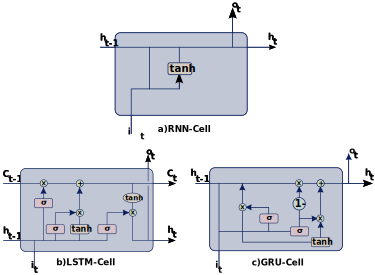
\includegraphics[width=\textwidth]{img/cells.pdf}
		\caption{The inner working of multiple recurrent cells}
		\label{fig:cells}
	\end{center}
\end{figure}
The inner workings of RNNs are illustrated in fig. \ref{fig:cells}a), where based on the input, the output, and the hidden state of the previous cell the output, the input, and the hidden state are computed. However, as previously outlined, more intricate RNN architectures exist to overcome the inherent problem of vanilla RNNs architectures. With long-short term memory, the problem of the vanishing gradient is elegantly addressed by using memory-cells, which have a self-connection of strength 1 and two auxiliary gating cells controlling the flow of information to and from each cell. This is in part achieved by closing or opening these gates. In other words, if the gates are closed, the gradients can flow freely without alteration during the entirety of the time-series, which is shown in fig. \ref{fig:cell}b). Technically, these gated cells decide about what to store, and when to allow reads, writes, and erases, and learn through an iterative process of choosing either to allow, leave, or delete the information then backpropagating the loss value and adjusting the weights accordingly\cite{kumar2018energy}. However, these gates cannot isolate the memory cell in practice, which doesn't free the LSTM from this problem in all situations. Nevertheless, the LSTM overcomes some synthetic problems with pathological long-range temporal dependencies, that were previously believed to be unredeemable by vanilla RNNs\cite{sutskever2013training}.\newline
Another variant of the LSTMs is gated recurrent units(GRUs), shown in \ref{fig:cells}c), which is relatively simpler to implement and reduces the computational overhead compared with LSTMs. However, the versatility against the problem of vanishing/exploding gradients is retained by simplifying the inner structure and resulting in leaning machines, that are computationally easier to train. This is due to the fact, that fewer computations are needed to optimize the model.\newline
Lastly, another approach is using bidirectional RNNs, where the input is fed from the beginning to the end and vice versa. This effectively increases the amount of information fed into the network and expands the context in which they operate. Moreover, the input flow in both directions allows for the preservation of future and past information thus improving the robustness of the model. This is achieved by using two separate hidden layers taking the input in two different directions. Next, the two hidden layers are both fed forward to the output layer\cite{graves2013hybrid}.
\section{RNN in Human Activity Recognition}
The interest in recurrent neural networks for research purposes in HAR resurged after the introduction of variants that overcome the inherent problems with them despite the additional computational costs. This is due to the fact, that they are more resilient and flexible and would enhance the quality of models based on these architectures. Rivera et al. used RNNs to perform this task by only feeding the model information about a hand. They saw in RNNs a huge chance for advancing the state-of-the-art in HAR, as these architectures forgo standard feature extraction methods and are advantageous due to the fact, that they have the ability to learn and extract hidden feature representation and classify the input accordingly. This is the case for all neural networks according to the team, but RNNs are more suitable due to their nature and their ability to properly process sequential data. For their study, they used a single IMU(Inertial Measuring Unit) to classify the activity of the hand, which is technically challenging with other machine learning approaches. To achieve this they used two LSTM layers and a softmax layer to generate p probability distribution and achieved very promising results in terms of accuracy and performance. However, they recognized that reducing confusion from transient states between activities by using an averaging filter of states, i.e. updating the current state based on the previous and next recognized states, leads to cleaner recognized activity logs by smoothing these transitions \cite{rivera2017recognition}.\newline 
Moreover, Vincent et al. used a shape-based method and LSTMs to perform human activity recognition based on a video input, which has intuitively a sequential nature. Thus makes LSTMs suitable architectures by virtue of the fact that they can retain extracted features sequentially and learn the temporal characteristics of human activities. In addition to that, the team acknowledged that they chose the LSTMs for their ability to add and remove information, consequently making them capable of learning long-term dependencies. However, these models aren't suitable for feature extraction from videos and images. Thus, they used a CNN to extract these features from the image sequences, which output is fed to the LSTM. Using this architecture the research team achieved promising results in terms of accuracy and robustness. Moreover, they experimented with bi-LSTMs also and conclude that they are better than normal LSTMs in terms of accuracy, but add more computational overhead\cite{vincent2020human}.\newline
